\chapter{HARDWARE AND SOFTWARE SPECIFICATION}
\label{ch:specifications}

\section{Hardware Requirements}
\hspace{2em}The physical implementation of VibeGuard is composed of carefully selected embedded electronics, transducers, actuators, precision mechanical fixtures, and circuit protection components designed to provide reproducible dynamic vibration data. Table~\ref{tab:components_required} presents the comprehensive hardware bill of materials and the functional role of each component as demonstrated during the official project review.

\begin{table}[H]
\centering
\caption{Hardware and tooling components required for the VibeGuard testbed}
\label{tab:components_required}
\small
\begin{tabular}{|l|p{10.5cm}|}
\hline
\textbf{Component} & \textbf{Functional Purpose in System} \\
\hline
ESP32 DevKit (7Semi) & Main controller executing high-speed SPI polling, zero-mean DC cancellation, Vector RMS, autotuning, and persistence filtering. \\
ADXL345 Accelerometer & 3-axis digital MEMS transducer measuring dynamic vibration up to $\pm 4g$ at 800\,Hz ODR over a 5\,MHz SPI bus. \\
RGB Status LED & Multi-state visual indicator displaying Normal (Green), Warning (Yellow), Alarm (Fast Red Strobe), Calibration (Blue), and Fault (Purple). \\
Resistors ($330\,\Omega$, $0.25$\,W) & Metal-film current-limiting resistors protecting ESP32 GPIOs and regulating RGB LED forward currents. \\
MB102 Breadboard / Baseplate & Prototype carrier and 10\,mm laminated acrylic platform providing rigid mechanical decoupling. \\
Jumper DuPont Wires & Low-noise interconnects for 5\,MHz SPI signals, 3.3\,V/5\,V logic power, and LED anodes. \\
Micro-USB Data Cable & Low-resistance cable providing 5\,V DC power and bi-directional 115200 baud serial telemetry to host. \\
12\,V N20 Gear Motor & Micro metal gear motor running at 600\,RPM (10.0\,Hz) providing periodic rotational unbalance excitation. \\
Custom 3D Mounts (FAB-01/02) & Monolithic PLA eccentric rotor cam arm and rigid gusseted bracket anchoring sensor directly to motor axis. \\
Host PC / Web Dashboard & Gateway running Node.js serial bridge and WebSocket server for live browser-based waveform and FFT plotting. \\
\hline
\end{tabular}
\end{table}

\subsection{Microcontroller Unit: 7Semi ESP32-DEVKIT-E}
\hspace{2em}The primary computational platform is the 7Semi ESP32-DEVKIT-E development board, integrating an Espressif ESP32-WROOM-32E system-in-package module. Table~\ref{tab:esp32_specs} summarizes its key architectural specifications.

\begin{table}[H]
\centering
\caption{7Semi ESP32-DEVKIT-E microcontroller technical specifications}
\label{tab:esp32_specs}
\begin{tabular}{|l|l|}
\hline
\textbf{Hardware Feature} & \textbf{Architectural Specification} \\
\hline
Core Architecture & 32-bit Dual-Core Xtensa LX6 Microprocessor \\
Clock Frequency & Up to 240\,MHz (Operated at 160\,MHz for thermal efficiency) \\
Internal SRAM & 520\,KB On-Chip SRAM \\
External Flash & 4\,MB SPI Flash Memory \\
USB-to-UART Interface & Silicon Labs CP2102 Bridge Controller \\
Onboard LDO Regulator & AMS1117-3.3 (800\,mA maximum rating) \\
General-Purpose Timers & Four 64-bit hardware timers with microsecond resolution \\
SPI Peripheral & Dedicated VSPI hardware controller \\
Operating Supply Voltage & 5.0\,V via Micro-USB (Regulated to 3.3\,V on-board) \\
\hline
\end{tabular}
\end{table}

\hspace{2em}The 7Semi board features the standard 38-pin DevKitC V4 physical header layout with a 22.86\,mm (0.90-inch) row pitch. When mounted across the central divider trench of a standard MB102 830-point solderless breadboard, one full row of tie-points remains accessible on either side, permitting direct breadboard jumper connections and diagnostic attachments.

\subsection{Triaxial Digital Accelerometer: Analog Devices ADXL345}
\hspace{2em}Mechanical vibrations are sensed using the Analog Devices ADXL345, an ultra-low power, 3-axis digital MEMS accelerometer. Table~\ref{tab:adxl345_specs} details its operational parameters.

\begin{table}[H]
\centering
\caption{Analog Devices ADXL345 accelerometer specifications}
\label{tab:adxl345_specs}
\begin{tabular}{|l|l|}
\hline
\textbf{Parameter} & \textbf{Configured Operational Value} \\
\hline
Measurement Dynamic Range & Configurable $\pm 2g, \pm 4g, \pm 8g, \pm 16g$ (Selected: $\pm 4g$) \\
Output Data Rate (ODR) & 800\,Hz (Bandwidth: 400\,Hz) \\
Digital Resolution & 11-bit Full Resolution Mode ($3.9\,\text{mg/LSB}$) \\
Communication Interface & 4-Wire SPI (Mode 3: $\text{CPOL}=1, \text{CPHA}=1$) \\
SPI Bus Speed & 5.0\,MHz Serial Clock \\
Operating Voltage & 3.3\,V DC (Current consumption: $\approx 140\,\mu\text{A}$) \\
Package / Mounting Pitch & Robocraze Breakout Board (15.0\,mm mounting hole pitch) \\
\hline
\end{tabular}
\end{table}

\subsection{Drive System and Power Infrastructure}
\hspace{2em}The mechanical vibration excitation is driven by a 12\,V DC N20 micro metal gear motor:
\begin{itemize}
    \item \textbf{Rotational Speed:} Nominally 600\,RPM at 12.0\,V DC, establishing a 10.0\,Hz fundamental rotational frequency ($1X$).
    \item \textbf{Output Shaft:} 3.0\,mm precision D-profile steel shaft (2.5\,mm flat thickness, 9.5\,mm usable length).
    \item \textbf{Mounting Bracket:} Heavy-duty U-profile steel bracket with M3 fasteners.
    \item \textbf{Power Adapter:} Regulated 12\,V DC 2.0\,A switched-mode power supply (SMPS) with a $5.5 \times 2.1$\,mm screw-terminal barrel connector.
\end{itemize}

\subsection{Mechanical Testbed and Custom 3D Printed Fixtures}
\hspace{2em}To ensure repeatable experimental conditions without acoustic rattling or structural resonance, custom mechanical fixtures were fabricated:

\begin{figure}[H]
\centering
\begin{tabular}{cc}
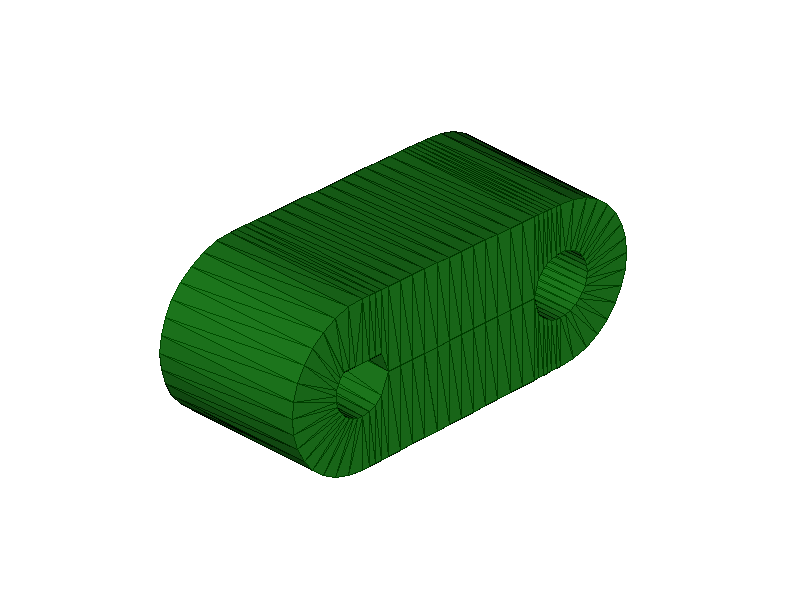
\includegraphics[width=0.46\textwidth]{fig/fig_rotor_arm_fab01.png} &
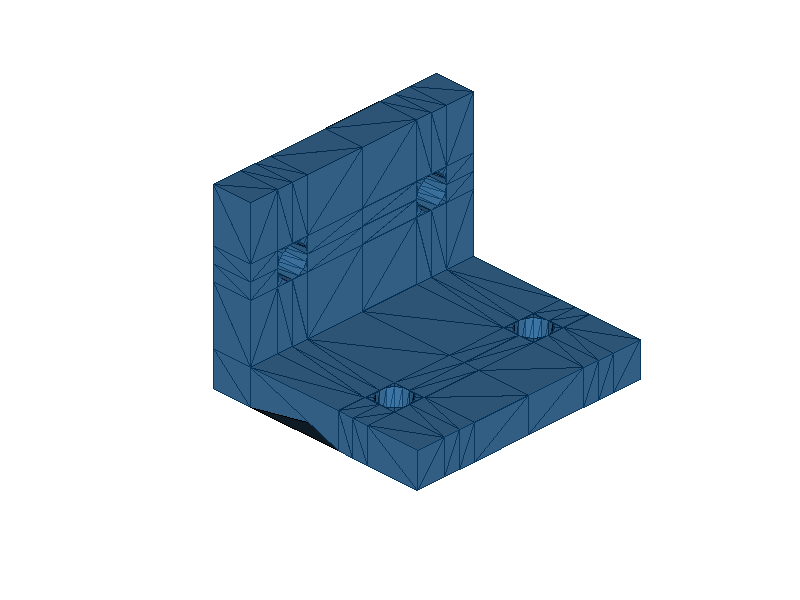
\includegraphics[width=0.46\textwidth]{fig/fig_sensor_mount_fab02.png} \\
\small (a) FAB-01 Rotor Cam Arm & \small (b) FAB-02 Rigid Sensor Mount \\
\end{tabular}
\caption{Monolithic 3D-printed mechanical components for the VibeGuard testbed}
\label{fig:cad_components}
\end{figure}

\begin{enumerate}
    \item \textbf{Laminated Acrylic Baseplate (150\,mm $\times$ 150\,mm $\times$ 10\,mm):} A 10\,mm thick dual-layer acrylic foundation machined with precision dual-datum through-holes. The plate rests on four 15\,mm silicone damping feet that isolate bench vibrations.
    \item \textbf{FAB-01 Eccentric Rotor Cam Arm:} A monolithic FDM 3D-printed PLA rotor component featuring a D-profile shaft bore (with $0.15$\,mm thermal shrinkage compensation) and an M3 counter-recess hole positioned at a 12.0\,mm pitch radius for unbalance mass attachment.
    \item \textbf{FAB-02 Rigid Sensor Mount:} A stiffened L-bracket with dual 45-degree gussets that rigidly clamps the ADXL345 PCB directly to the baseplate adjacent to the motor, maintaining high mechanical coupling across the 0--400\,Hz bandwidth.
\end{enumerate}

\begin{figure}[H]
\centering
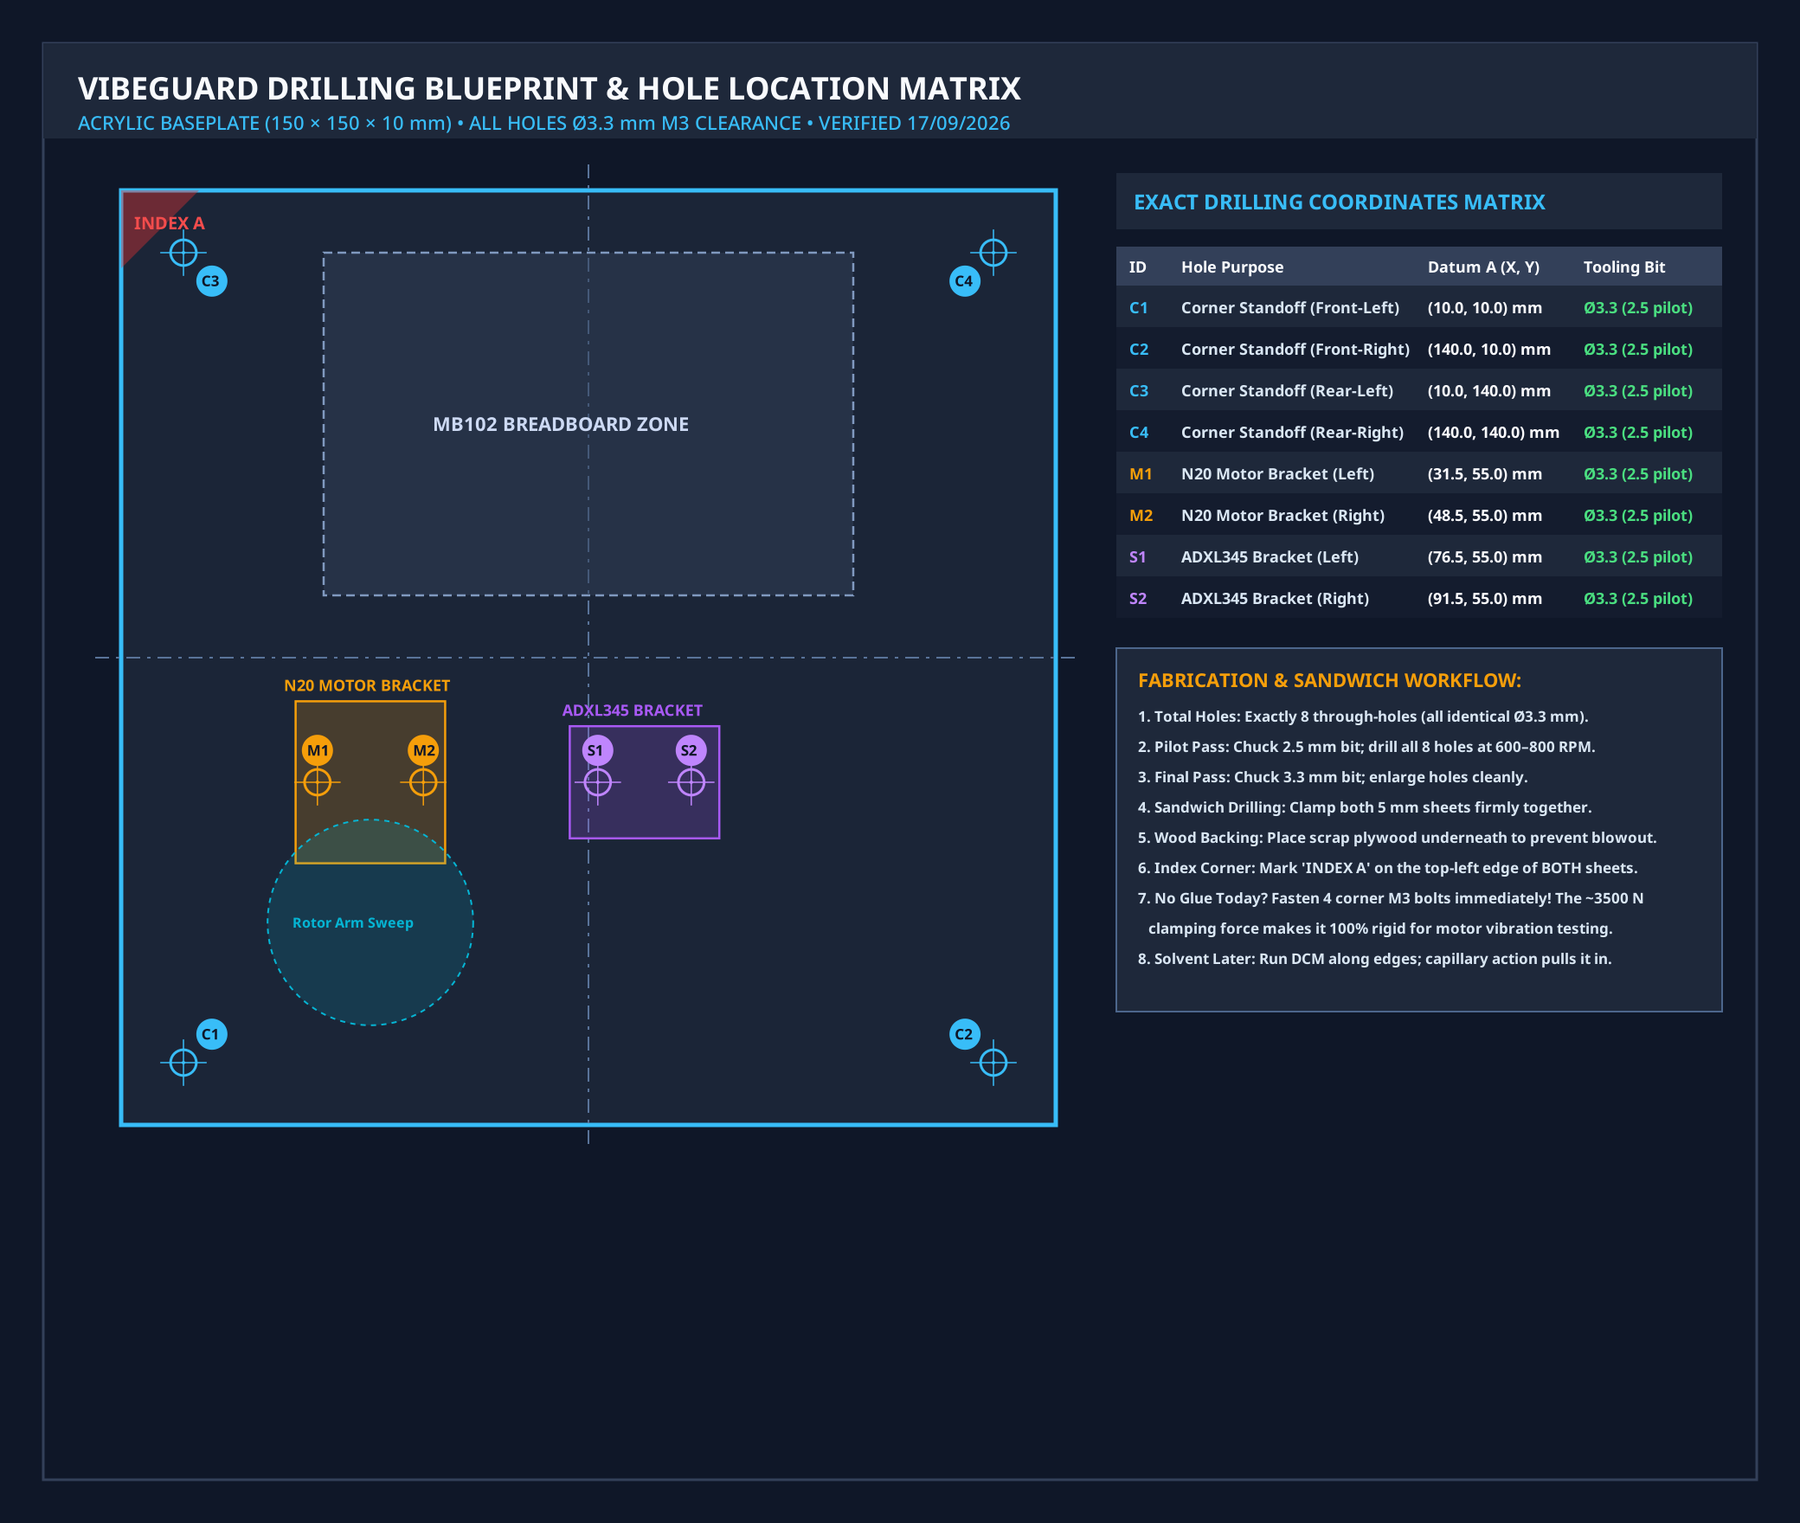
\includegraphics[width=0.88\textwidth]{fig/fig_baseplate_blueprint.png}
\caption{Precision drilling blueprint and dimensional layout for the 10\,mm acrylic baseplate}
\label{fig:baseplate_blueprint}
\end{figure}

\subsection{Circuit Protection and Status Indication Components}
\begin{itemize}
    \item \textbf{Flyback Diode:} 1N4007 silicon rectifier diode (1000\,V PIV, 1.0\,A continuous).
    \item \textbf{Decoupling Capacitors:} $100\,\mu\text{F}$ 25\,V radial electrolytic capacitor and $100\,\text{nF}$ multi-layer ceramic capacitor (MLCC).
    \item \textbf{Current Limiting Resistors:} Three $330\,\Omega$ $0.25$\,W metal-film resistors for the RGB channels.
    \item \textbf{RGB LED:} Common-cathode 5\,mm diffused LED (Green: Pin 25, Blue: Pin 26, Red: Pin 27).
    \item \textbf{Safety Switch and Fuse:} KCD1 2-pin rocker switch and 1.0\,A 250\,V fast-blow cartridge fuse in an enclosed chassis holder.
\end{itemize}

\section{Software Requirements}
\hspace{2em}The software infrastructure comprises embedded C/C++ firmware running bare-metal on the ESP32, accompanied by host-side diagnostic and visualization applications.

\subsection{Programming Language and Compilation Toolchain}
\begin{itemize}
    \item \textbf{Language:} C++17 standard, utilizing deterministic fixed-size buffers and avoiding dynamic heap allocations in the real-time loop.
    \item \textbf{Toolchain:} Espressif \texttt{xtensa-esp32-elf-g++} compiler with \texttt{-O2} optimization flags, managed under the Arduino-ESP32 Core (v2.0.14+) / ESP-IDF framework.
\end{itemize}

\subsection{Host Telemetry and Real-Time Web Dashboard}
\begin{itemize}
    \item \textbf{Serial-to-WebSocket Bridge:} A lightweight Node.js daemon (\texttt{server.js}) interfaced with the ESP32 via USB serial at 115200 baud, converting raw JSON telemetry into bi-directional WebSocket frames.
    \item \textbf{Interactive Web Dashboard:} A responsive browser-based user interface utilizing Chart.js to render real-time time-series RMS vibration curves, rolling FFT magnitude spectra, state status banners, and dynamic anomaly gauges.
\end{itemize}

\subsection{Firmware Architecture and Modular Organization}
The embedded codebase is structured into four cohesive modules:
\begin{enumerate}
    \item \textbf{ADXL345 SPI Driver (\texttt{adxl345\_spi}):} Implements low-level register read/write methods over the 5\,MHz SPI bus, device ID validation, and burst 6-byte acceleration reads.
    \item \textbf{DSP Feature Extractor (\texttt{VibeGuardEngine}):} Implements rolling mean DC cancellation, 3-axis Vector RMS computation, adaptive autotuning, and Radix-2 Cooley-Tukey FFT with Hann windowing.
    \item \textbf{State Machine Controller (\texttt{state}):} Implements the $K$-of-$M$ persistence circular buffer and evaluates transition rules between \texttt{BOOT}, \texttt{CALIBRATING}, \texttt{NORMAL}, \texttt{WARNING}, \texttt{ALARM}, and \texttt{SENSOR\_FAULT}.
    \item \textbf{Main Controller (\texttt{VibeGuard\_Autotune\_Synchronized.ino}):} Manages timer interrupts, acquisition pacing at $1250\,\mu\text{s}$, RGB LED actuation, and telemetry formatting.
\end{enumerate}

\section{Summary}
\hspace{2em}This chapter specified the hardware components, mechanical fixtures, and software environments comprising VibeGuard. The combination of the 7Semi ESP32-DEVKIT-E, ADXL345 SPI accelerometer, precision acrylic testbed, custom 3D-printed mounts, modular C++ firmware, and real-time host web dashboard establishes a robust, reproducible platform for edge vibration monitoring.
\clearpage
